\chapter{SubVis}

Nachfolgend wird das Programm \emph{SubVis} spezifiziert und dessen Architektur vorgestellt.
Außerdem wird auf die konkrete Implementierung, Tools, Bibliotheken und Dokumentation eingegangen.

\section{Anforderungen}

\begin{itemize}
 \item Architektur
 \begin{itemize}
 	\item Erweiterbarkeit durch andere Algorithmen und Visualisierungen mittels Plugins.
 	\item Plugins können eigene GUI-Elemente in dafür vorgesehenen Bereichen zeichnen.
 	  \item Anwendung von verschiedenen Algorithmen auf den jeweiligen Polygonnetzen
 	  \item Rückgängig/Wiederherstellen von Operationen
 \end{itemize}
 \item GUI
  \begin{itemize}
 	\item Darstellung des Kontrollnetzes
 	\item Darstellung der Limesfläche
 	\item Rotation des Objektes
 	\item Translation des Objektes
 	\item Skalierung des Objektes
 	\item Beleuchtung der Oberfläche des Netzes, um Glattheit bewerten zu können
 	\item Edit-Modus: Verschieben eines Punktes anhand seiner Flächennormalen
 	\item Abbrechen von langlaufenden Unterteilungsschritten
    \item Statistik des Polygonnetzes anzeigen
    \item Splitscreen zur Darstellung von zwei Polygonnetzen
 \end{itemize}
 \item Dateiformate / IO
 \begin{itemize}
 	\item OFF-Format und NOFF (mit Farben/Normalen)
 	\item Laden und Speichern von Polygonnetzen
 \end{itemize}
 \item Unterteilungsalgorithmen
 \begin{itemize}
 	\item Catmull-Clark
 	\item Loop
 	\item Doo-Sabin
 	\item Butterfly
 	\item Modified Butterfly
 \end{itemize}
 \item Funktionen
 \begin{itemize}
  \item Variable Anzahl von Unterteilungsschritten
  \item Beleuchtungsmodus wählbar

 \end{itemize}
\end{itemize}

\section{Tools und Bibliotheken}

\emph{SubVis} greift auf die Bibliotheken Qt, libQGLViewer, OpenGL Mathematics, astyle, Surface\_mesh, OpenGL und Doxygen zurück.
Die verwendeten Versionen sind in \autoref{tab:versionen} ersichtlich.

\begin{table}[h]
\center
\caption{Versionen der Bibliotheken}
\label{tab:versionen}
\begin{tabular}{c|c}
Bibliothek & Version\\
\hline
Qt & 5.4.1\\
libQGLViewer & 2.6.1\\
Surface\_mesh & 1.0\\
OpenGL & 10.1.3-0ubuntu0.4\footnote{Ubuntu Paket mesa-common-dev}\\
Doxygen & 1.8.6\\
GLM & libglm-dev 0.9.5.1-1\\
Astyle & 2.03\\
\end{tabular}
\end{table}

\section{Entwicklungsprozess}

Um eine gemeinsame Entwicklungsumgebung zu schaffen, wurden gewisse Bibliotheken, Tools und Plattformen spezifiziert.
Dies betrifft einerseits die Bibliotheken und Tools aus \autoref{tab:versionen}.
Andererseits auch das Betriebssystem, Versionsverwaltung, IDE und Programmiersprachenstandard.

Als Betriebssystem wird Ubuntu 14.04 LTS verwendet. 
Zum Projektabschluss wird jedoch eine plattformunabhängige Anwendung angestrebt.
Die Sprachfeatures von C++ sollen maximal dem C++11 Standard entsprechen.
Als Versionsverwaltung wird Git in Verbindung mit dem Git-Server des IOS an der HTWG eingesetzt. 

Die Entwicklung findet auf dem \emph{develop}-Branch und eventuellen Feature-Branches statt.
Dabei sollte ein Branch pro Feature erstellt werden und erst dann in den develop-Branch gemergt werden, wenn das Feature funktioniert.
Als IDE wird der vorgestellte Qt Creator verwendet.

Zur Formatierung des Quellcodes wird astyle verwendet. 
Die Options-Datei style.astylerc definiert für das Projekt die Formatierungsregeln. 

Als Style Guide für den Programmierstil wird der Google C++ Style Guide verwendet \cite{GsgC++}.
Abweichungen sind jedoch in begründeten Fällen erlaubt und werden dokumentiert.

Das Projekt teilt sich in zwei Verzeichnisse auf: \emph{SubVis} und \emph{dev-doc}.
\emph{SubVis} enthält die gleichlautende Anwendung als Qt-Projekt und unterteilt sich noch in die Ordner \emph{app}, \emph{lib} und \emph{objs}.
\emph{app} enthält die Anwendungsteile die selbst entwickelt werden,
\emph{lib} die Drittherstellerbibliotheken und \emph{objs} 3D-Modelle zum Testen.
\emph{dev-doc} dient der weiterführenden Dokumentation.
Das Verzeichnis enthält z. B. Diagramme, diesen Bericht und andere hilfreiche Dokumente zur Entwicklung.

\section{Grafische Oberfläche}

\begin{figure}
  \centering
  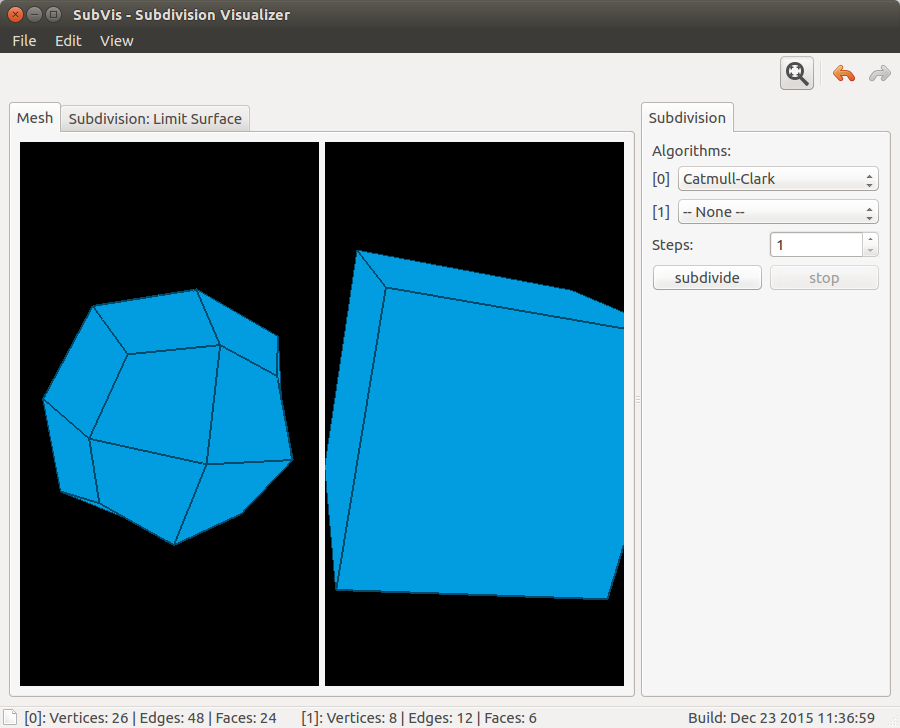
\includegraphics[width=\textwidth]{content/media/subvis_mesh.png}
  \caption{Kontrollnetz in SubVis}
  \label{fig:subvis_mesh}
\end{figure}

Die grafische Oberfläche bietet eine aufgeräumte Ansicht der wichtigsten Elemente (siehe \autoref{fig:subvis_mesh}). 
Im oberen Bereich findet sich die Menüleiste mit Dateioperatoren, Editierwerkzeugen und Optionen zur Steuerung der Ansicht.
Darunter befindet sich eine Toolbar, welche häufig verwendete Aktionen enthält.
Am unteren Ende des Fensters ist eine Statusleiste integriert, welche Informationen über das Polygonnetz anzeigt (Anzahl an Knoten etc.).
Der Hauptbereich der Anwendung ist die Darstellung von zwei Viewern, welche separat bedient werden können und verschiedene Zustände der Polygonnetze darstellen können.
Diese unterstützen Rotation, Zoom und Translation.
Über die Tabs darüber kann zwischen der generischen Polygonnetzansicht und Plugin-spezifischen Ansichten umgeschaltet werden.
Geladene Plugins werden auf der rechten Seite in Form von Tabs angezeigt.
Diese besitzen eine jeweils individuelle GUI.

Die Anwendung bietet eine Rückgängig/Wiederherstellen Funktion in Form von zwei Pfeilen. Durch diese können Modifikationen an den Polygonnetzen rückgängig gemacht werden.
Manchmal ist es von Vorteil, wenn die beiden getrennten Viewer sich synchronisieren.
Dies kann über die Funktion \enquote{Synchronize Views} erreicht werden. 
Nach der Aktivierung bewegen sich die Kameras der beiden Viewer absolut synchron.
Eine Art \enquote{ablenkungsfreier Modus} lässt sich erreichen, in dem der zweite, rechte Viewer ausgeblendet wird. 
Zusätzlich kann die rechte Tableiste der Plugins ausgeblendet oder verkleinert werden.

Alle Menü- und Toolbar-Elemente lassen sich auch über Tastenkürzel erreichen.

\begin{figure}
  \centering
  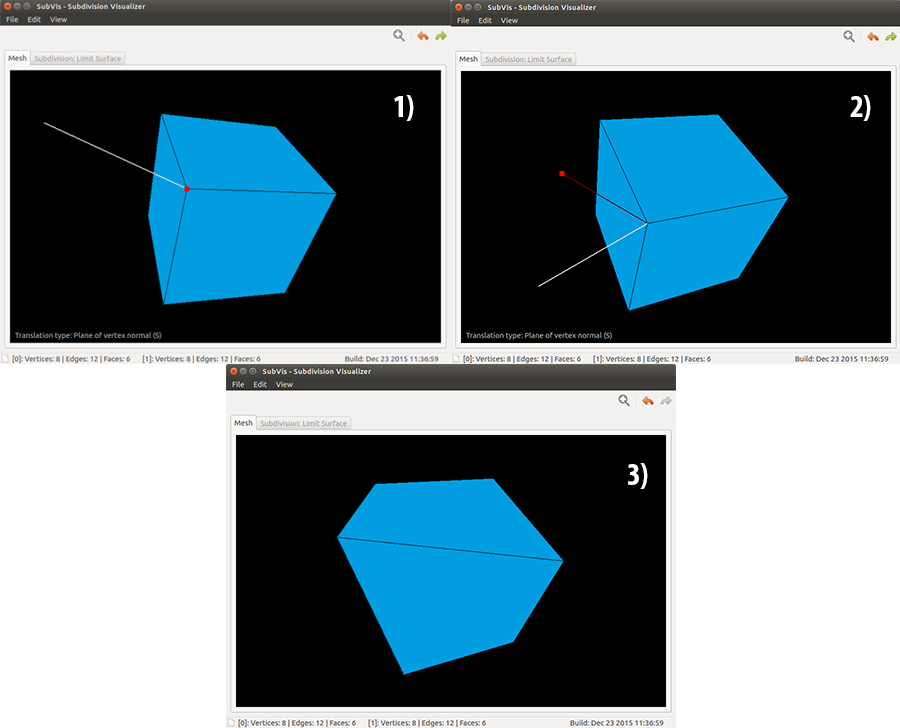
\includegraphics[width=\textwidth]{content/media/subvis_edit.png}
  \caption{1) Selektion eines Vertex 2) Translation 3) Resultierendes Polygonnetz}
  \label{fig:subvis_edit}
\end{figure}

Durch Aktiveren des Editiermodus (siehe \autoref{fig:subvis_edit}) wird in den ablenkungsfreien Modus geschaltet.
Nach Doppelklick auf einen Vertex oder dessen unmittelbare Umgebung wird dieser selektiert, vergrößert in rot dargestellt und dessen Normale in weiß eingezeichnet (siehe Schritt 1 von \autoref{fig:subvis_edit}).
Während der Vertex mittels STRG+linke Maustaste im Raum bewegt wird, wird zusätzlich eine rote Linie zwischen der Ursprungsposition und der neuen Position angezeigt (siehe Schritt 2 von \autoref{fig:subvis_edit}).
Dabei bewegt sich der Vertex lediglich auf der Ebene, die durch die Normale des Vertex definiert wird.
Damit eine beliebige Positionierung im Raum möglich ist, kann zwischen der Ebene der Normale und einer Ebene, die orthogonal zur dieser steht mit der Taste S umgeschaltet werden.
Durch erneutes Doppelklicken (an einer beliebigen Stelle) wird der Editiervorgang beendet und das veränderte Polygonnetz dargestellt (siehe Schritt 3 von \autoref{fig:subvis_edit}).


\section{Implementierung}

In diesem Kapitel wird auf die konkrete Architektur, Implementierung und detaillierte Entwicklungsentscheidungen eingegangen.

\subsection{Gesamtarchitektur}

Die grundlegende Architektur ist in \autoref{fig:subvis_architektur} als UML-Komponentendiagramm dargestellt. 
Grundsätzlich wird auf eine Model-View Architektur gesetzt.

Die Model-Komponente kapselt eine Datenstruktur, die das Polygonnetz enthält und bietet grundlegende Polygonnetzoperationen und Import bzw. Persistenzoperationen.
Sie sendet außerdem bei Modifikation eines Polygonnetzes ein Signal an alle Listener aus.
Der Zugriff auf das Polygonnetz ist nur lesend möglich, jeder schreibende Zugriff muss zuerst eine Kopie erstellen und diese nach der Modifikation wieder in die Model-Komponente laden.
Dadurch wird ein gewisser Grad an Immutabilität erreicht, welcher die Robustheit der Anwendung erhöht.

Die View-Komponente ist für die Darstellung/Editieroperationen verantwortlich.
Diese verbindet auch die Signale der anderen Komponenten mit den Slots der Plugins bzw. Model-Komponente.
Zusammengesetzt aus den Komponenten \emph{tabs\_plugins} (GUI-Elemente der einzelnen Plugins), \emph{toolbar} (Werkzeugleiste), \emph{tabs\_viewer} (generischer Polygonnetz-Viewer und Plugin-spezifischer Viewer) und \emph{menu\_bar} (Menüleiste) bildet die View-Komponente alle grundlegenden Darstellungsoperationen ab.
Die Komponente \emph{tabs\_viewer} enhält einerseits einen generischen Viewer, der das Polygonnetz rendert und einen Editiermodus bereitstellt. 
Andererseits einen Viewer, dessen Darstellung durch das aktive Plugin gesteuert wird.
Dies erlaubt den Plugins maximale Freiheit bezüglich der Darstellung, da so das Polygonnetz gerendert werden kann aber auch eine völlig unabhängige Darstellung erfolgen kann.
Durch Verbindung mit den Signalen der Model-Komponente, wird auf Veränderungen im Polygonnetz reagiert.

Plugins werden von einem \emph{PluginManager} verwaltet, bei welchem sich die Plugins zuvor registriert werden müssen.
Dieser erlaubt die Verwendung von mehreren Plugins, wovon jedoch nur eines zu einem Zeitpunkt aktiv sein kann (durch Auswahl des jeweiligen Tabs in der GUI).
Plugins werden auch über Veränderungen in der Model-Komponente benachrichtigt.
Sie können auch ein Signal aussenden, um anzuzeigen, dass sie ein erneutes Rendering durchführen möchten.
Dieses Signal wird von der View-Komponente erkannt und in einen Aufruf der draw-Methode des Plugins umgesetzt.
Die Plugins erhalten die Möglichkeit eine eigene GUI zu erstellen und ein spezifisches Rendering durchzuführen.

\begin{figure}
  \centering
  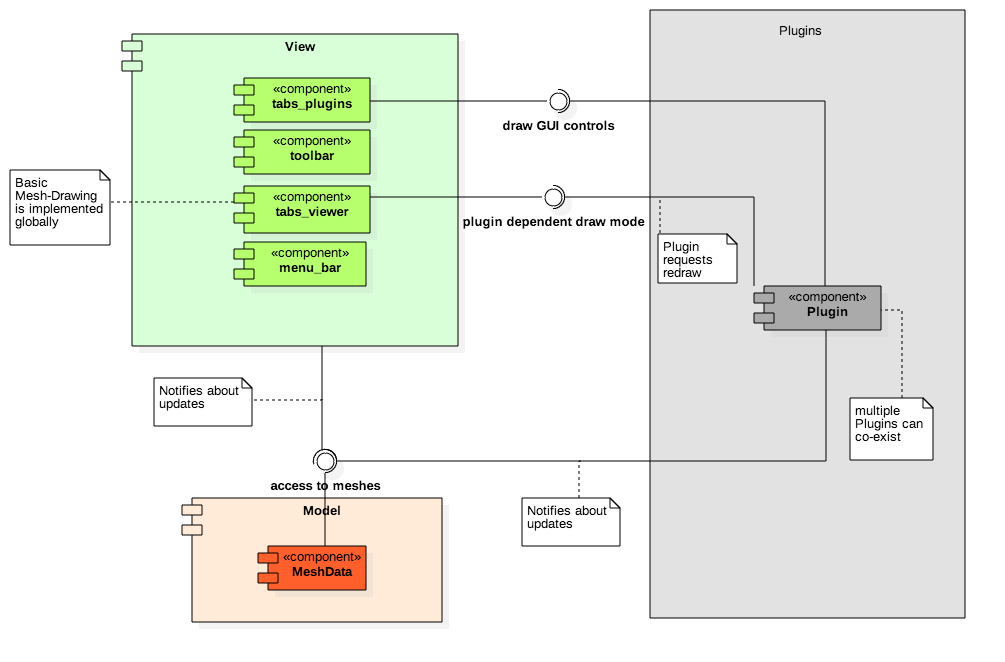
\includegraphics[width=\textwidth]{content/media/subvis_architektur.png}
  \caption{Gesamtarchitektur von SubVis}
  \label{fig:subvis_architektur}
\end{figure}


\subsection{Speicherverwaltung}

In C++ Programmen muss eine Auseinandersetzung mit den Themen Speicherverwaltung und Ownership erfolgen.
Der C++11 Standard bietet die Möglichkeit mit den Typen \emph{unique\_ptr} und \emph{shared\_ptr} die Speicherverwaltung automatisch und explizit zu machen.
Im Gegensatz zu einer manuellen Speicherverwaltung werden somit mehrfache oder fehlende \emph{free} Aufrufe verhindert, was die Stabilität des Systems erhöht.
Der Typ unique\_ptr kapselt einen Zeiger und gibt dessen Speicher frei, sobald die Variable ihren Gültigkeitsbereich verlässt oder neu zugewiesen wird \cite{C++Ref}. 
Somit wird das Konzept des eindeutigen Ownerships einer Ressource umgesetzt.
Dahingegen erlaubt der Typ shared\_ptr mehrere Besitzer und gibt den Speicher der Ressource erst frei, sobald die Variable durch keinen Besitzer mehr erreichbar ist.
Dadurch kann der Ownership auf mehrere Instanzen verteilt werden, die alle gleichberechtigte Besitzer sind.

SubVis benutzt ausschließlich diese beiden Typen zur Speicherverwaltung.
Ausnahmen sind lediglich Container-Typen, die eine ähnliche Semantik haben und Ressourcen die von Qt verwaltet werden.
Die von Qt verwalteten Ressourcen werden automatisch bei Beendigung des Programms freigegeben, da diese eine Parent-Child-Beziehung besitzen und mit Zerstörung des Hauptfensters von Qt entsprechend behandelt werden.
Die durchgehende Verwendung von unique\_ptr und der Move-Semantik in C++11 wird jederzeit deutlich, welches Objekt Besitzer einer Ressource ist.

\subsection{Model}

\begin{figure}
  \centering
  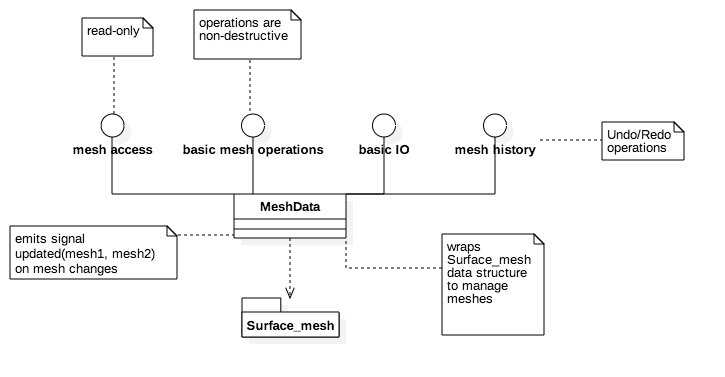
\includegraphics[width=\textwidth]{content/media/subvis_architektur_model.png}
  \caption{Architektur der Model-Komponente von SubVis}
  \label{fig:subvis_architektur_model}
\end{figure}

\autoref{fig:subvis_architektur_model} zeigt die Klassen der Model-Komponente.
Die Schnittstelle ist in der Abbildung in mehrere Teilschnittstellen aufgegliedert, um die Komponenten verständlicher darzustellen.
Als Datenstruktur zur Verwaltung der Polygonnetze wird Surface\_mesh verwendet.
Diese wird auch als Ein- und Ausgabetyp der Model-Komponente benutzt.

Grundsätzlich verwaltet die Komponente stets zwei Instanzen der Datenstruktur.
Diese werden über die Nummerierung 0 und 1 (als index bezeichnet) identifiziert.
Jede Anfrage nach der Datenstruktur wird mit einem Paar (std::pair) dieser beiden Instanzen beantwortet. 
Dabei handelt es sich um einen lediglich lesenden Zugriff (const).
Diese Entscheidung wurde zugunsten eines besser nachvollziehbaren Programmflusses getroffen, da Immutabilität Software einfacher und robuster macht.
Wenn ein Polygonnetz bzw. eine Kopie davon verändert wurde, dann kann dieses in die Model-Komponente mit der IO-Schnittstelle geladen werden.
Dies muss immer als Paar erfolgen. 
Jedoch wird aus Komfort eine Methode angeboten, eine einzelne Instanz zu laden, wobei diese einfach dupliziert wird.
Des Weiteren können Dateien im Format obj, off und stl geladen bzw. im Format off gespeichert werden.

Über Veränderungen der Datenstruktur werden andere Komponente informiert, in dem das Signal \emph{updated} ausgesendet wird. 
Diese enthält als Parameter beide aktuellen Datenstrukturinstanzen.

Die Komponente realisiert darüber hinaus eine Historie der Instanzen.
Es wird eine festgelegte Anzahl an Paaren von Instanzen im Hauptspeicher gehalten.
Mit den entsprechenden Methoden kann in dieser Historie beliebig vor und zurück gesprungen werden.
Dies ermöglicht die einfache Realisierung einer Rückgängig/Wiederherstellen Funktion.
Die Implementierung nutzt einen std::vector und einen Index, um in diesem Array vor und zurück zu springen.
Bei jedem neuen Historieeintrag wird der Speicher der Datenstrukturen optimiert durch Aufruf einer Garbage-Collection Funktion.
Beim Hinzufügen von neuen Paaren in die Historie können sich zwei Fälle ergeben:

\begin{itemize}
\item[a)] Der Index zeigt auf ein Element vor der neuesten Historie (zuvor wurde zurück gesprungen).
\item[b)] Die Historie hat die maximale Kapazität erreicht.
\item[c)] Der Index zeigt auf das aktuellste Element und die Historie hat noch Kapazität.
\end{itemize}

Im Fall c) ist nichts zu machen, außer das Paar hinzuzufügen und den Index zu erhöhen.
Im Fall a) müssen alle Einträge ab dem Index bis zum aktuellsten Element entfernt werden. 
Dadurch ist auch garantiert, dass auf jeden Fall ein Element Platz hat.
Bei Fall b) müssen Elemente entfernt werden. 
Dabei werden alle Elemente gelöscht, bis auf das erste Element (leere Polygonnetze) und das zweite Element (zuletzt geladende, unveränderte Polygonnetze).
 

\subsection{View}

\begin{figure}
  \centering
  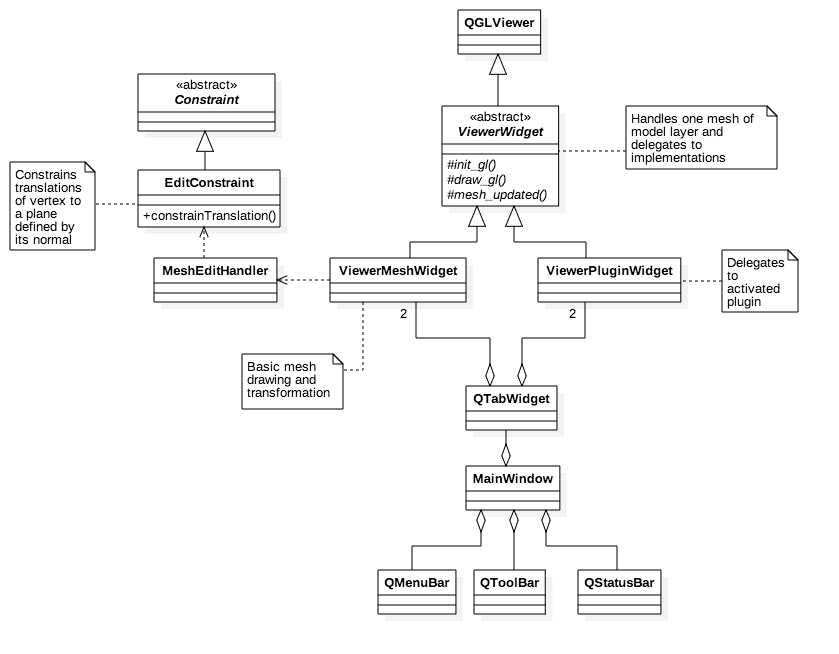
\includegraphics[width=\textwidth]{content/media/subvis_architektur_view.png}
  \caption{Architektur der View-Komponente von SubVis}
  \label{fig:subvis_architektur_view}
\end{figure}

Die View-Komponente setzt wo möglich auf vorhandene Qt-Klassen oder erweitert diese (siehe \autoref{fig:subvis_architektur_view}).
Die zentrale Klasse ist \emph{MainWindow}. 
Sie wird zum Teil von Qt aus einer Formulardatei generiert (in einem ui\_mainwindow.h Header) und zum Teil manuell implementiert.
MainWindow besteht aus den UI-Klassen für Menü-, Werkzeug- und Statusleiste.
Des Weiteren aus zwei QTabWidget.
Eines davon wird als Container für die Plugin-GUIs benutzt (pro Plugin ein Tab).
Das andere ist der Container für die beiden Viewer-Tabs \emph{Kontrollnetz-Rendering} und \emph{Plugin-spezifisches Rendering}.
Der aktuell aktive Plugin-Tab wird automatisch dem Plugin-spezifischen Viewer-Tab zugeordnet und kann eine eigene Beschriftung setzen.
Für die Realisierung von zwei simultan aktiven Viewern pro Tab wird ein QSplitter eingesetzt, welcher die verfügbare Fläche in zwei gleiche Teile unterteilt.

\subsubsection{ViewerWidget}

Die Oberklasse ViewerWidget stellt einen generischen Viewer für SubVis dar.
Sie erweitert QGLViewer und verbindet sich mit dem updated Signal der Model-Komponente.
Mittels des Template-Patters können die Unterklassen von ViewerWidget ihre OpenGL Draw-Calls ausführen.
ViewerWidget initialisiert zuvor einige Maus-Bindings, kümmert sich um das Layout und reicht das konkrete Polygonnetz an die Unterklasse weiter.
Ein Viewer wird stets mit einer ID instanziert, die den Index des Polygonnetzes (vgl. Model-Komponente) spezifiziert.
Somit müssen die Unterklassen lediglich ein einzelnes Polygonnetz verwalten und nicht zwischen beiden unterscheiden.

\subsubsection{ViewerPluginWidget}

Diese Klasse ist im Prinzip lediglich ein dünner Wrapper um ein Plugin und delegiert alle nötigen Aufrufe an das Plugin weiter.

\subsubsection{ViewerMeshWidget}



\subsection{Plugins}

Manager etc. DIAGRAMM




\section{Erstellung eines Plugins}

\section{Dokumentation}

Die Dokumentation besteht aus diesem Bericht sowie der finalen schriftlichen Ausarbeitung am Ende des 2. Semesters.
Diese Ausarbeitung soll die theoretischen Hintergründe erklären, sowie auf die Entwicklungsprozesse inkl. Vergleich und Entscheidungen für spezifische Technologien eingehen.
Ziel ist es, dem Leser eine Top-Down-Ansicht auf das Projekt zu verschaffen.
Es wird bewusst auf eine detaillierte Quellcodedokumentation in der Ausarbeitung verzichtet, um die Dokumentation nahe am Quellcode und aktuell zu halten.

Durch Quellcodedokumentierung sollen Entwickler befähigt werden schnell in das Projekt einsteigen zu können und das Programm weiter zu entwickeln bzw. durch Plugins zu erweitern.
Insbesondere bei den Plugins soll ein kurzes Tutorial erstellt werden, welches an die Plugin-Entwicklung heranführt. 
Des Weiteren soll ein kleines, gut dokumentiertes Plugin entstehen, um den prinzipiellen Aufbau zu veranschaulichen.
Wenn zu viel dokumentiert wird, veraltet diese schneller.
Deswegen soll \emph{sinnvoll} und \emph{angemessen} dokumentiert werden.
Dies bedeutet öffentliche APIs, wenn notwendig, detailliert und ausführlich zu dokumentieren und selbsterklärende Funktionen etc. nicht unnötig zu dokumentieren.
Grundsätzlich soll der Quellcode selbst schon als Dokumentation dienen können.
Zusätzlich finden sich beim Quellcode README-Dateien, die genaue Details über die verwendeten Funktionen, Build-Anleitungen und die Projektstruktur erläutern.

\section{Buildprozess}

Linken der Bibliotheken

\section{Installation}

\section{Benutzerhandbuch}
































